\section{Endliche Zustandsautomaten, Finite State Machine}
\subsection{Grundlegende Eigenschaften}
Eine FMS ist ein Geschlossenes Modell mit einer endlichen Anzahl von Zust�nden,
Zustands�berg�ngen und Aktionen.\\
\textbf{Sinn:} Mathematische Abstraktion, Grundlage theoretischer
Betrachtungen, Ausgangspunkt systematischer parktischer Realisierung.\\
\textbf{Anweundungen:} Informatik (Parser, Compiler, Game)\\
Technik, digitale Schaltungen (Kaffee-Automat, Parkticket, \ldots)\\
Kommunikationstechnik (Protokolldesign)\\
  \subsubsection{Grundstruktur}
  \begin{multicols}{3}
    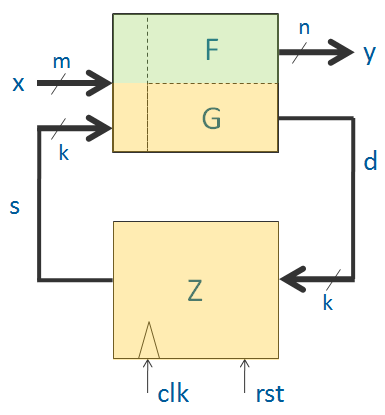
\includegraphics[width=0.2\textwidth]{pics/fsm_grundlage}
    \textbf{Kombinatorische Logik F/G}\\
    Generiert Ausg�nge\\ und Folgezustand.\\
    F = Funktion f�r Ausg�nge\\
    G = Funktion f�r Speicheransteuerung\\
    \textbf{Zustandsregister Z}\\
    Z = Zustansspeicher/register\\
    Sequentieller Teil des Systems,\\
    speichert aktuellen Zustand.\\
    \textbf{Signale}\\
    x = Eingangsvektor\\
    m = Anzahl Eing�nge\\
    y = Ausgangsvektor\\
    n = Anzahl Ausg�nge\\
    s = Zustandsvektor\\
    d = Folgezustand\\
    \textbf{Memory}\\
    k = Anzahl Speicherstellen\\
    
  \end{multicols}
  %Bild V4F7
\subsection{Mealy, Moore und Medwedjew}
\begin{tabular}{|p{6cm}|p{6cm}|p{6cm}|}
  \hline
  \textbf{Mealy-System} & \textbf{Moore-System} & \textbf{Medwedjew-System} \\
  \hline
  Grundsystem; komb. Logik F/G in zwei separate Bl�cke aufgeteilt & Wert der
  prim�ren Ausg�nge ist nur vom aktuellen Zustand des Systems abh�ngig. &
  Spezialfall des Moore-Systems: Prim�re Ausg�nge entsprechen dem Zustandsvektor \\
  \hline
  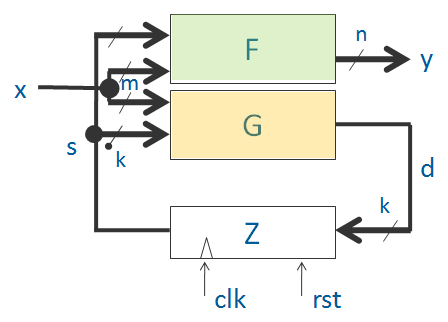
\includegraphics[width=0.3\textwidth]{pics/fsm_mealy} &
  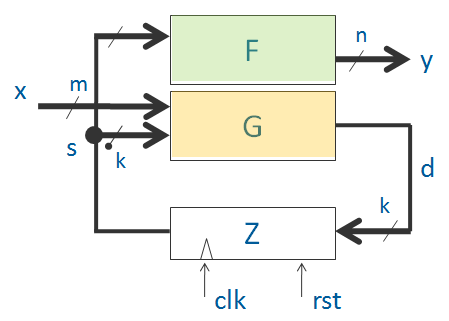
\includegraphics[width=0.3\textwidth]{pics/fsm_moore} &
  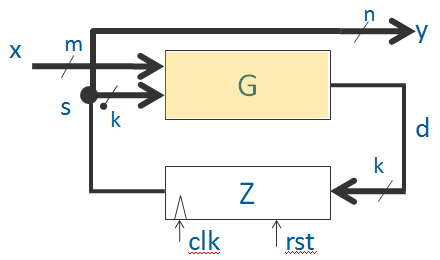
\includegraphics[width=0.3\textwidth]{pics/fsm_medwedjew} \\
  \hline
  Ausg�nge h�ngen vom momentanen Zustand und den aktuellen Eing�ngen ab.
  & Ausg�nge h�ngen nur vom momentanen Zustand ab und �ndern mit der
  Clock-Flanke & Die prim�ren Ausg�nge entsprechen dem Zustandsvektor.
  Ausgangsfunktion F degeneriert auf 1. \\
  \hline
  $ y[i] = F(x[i],x[i]) $ & $ y[i] = F(s[i]) $ & $ y[i] = s[i] := G(x[i-1],y[i-1]) $ \\
  $ d[i] = s[i+1] := G(x[i],s[i]) $ & $ d[i]=s[i+1] := G(x[i],s[i]) $ & $ 
  s[i+1]:=G(x[i],s[i])$ \\
  \hline
  Entwurf mit asynchronem Output. Ausgabe unabh�ngig vom Clock. & Allgemeiner Prototyp eines synchronen, sequentiellen Entwurfes. & Ausg�nge
  entsprechen den Zust�nden.\\
  \hline
  Lange Signalpfade! & Verz�gerung Latenzzeit & Zust�nde m�ssen gleich codiert
  werden wie Ausgangssignale\\
  \hline
  Mausefalle & & Die meisten Counter \\
  \hline
  %Code zu einzelnen Varianten hinzuf�gen V4 ab seite 21
\end{tabular}
